\documentclass[english,notitlepage]{revtex4-1}  % defines the basic parameters of the document
%For preview: skriv i terminal: latexmk -pdf -pvc filnavn



% if you want a single-column, remove reprint

% allows special characters (including æøå)
\usepackage[utf8]{inputenc}
\usepackage[english]{babel}


\usepackage{physics,amssymb}  % mathematical symbols (physics imports amsmath)
\include{amsmath}
\usepackage{graphicx}         % include graphics such as plots
\usepackage{xcolor}           % set colors
\usepackage{hyperref}         % automagic cross-referencing (this is GODLIKE)
\usepackage{subcaption}
\usepackage{listings}         % display code
\usepackage{float}
\usepackage{enumitem}
%\usepackage[section]{placeins}
\usepackage{algorithm}
\usepackage[noend]{algpseudocode}
\usepackage{tikz}
\usetikzlibrary{quantikz}

\hypersetup{
    colorlinks,
    linkcolor={red!50!black},
    citecolor={blue!50!black},
    urlcolor={blue!80!black}}



\begin{document}

\title{Project 2}
\author{Alessio Canclini, Filip von der Lippe}
\date{\today}
\noaffiliation                            % ignore this, but keep it.


\maketitle

\textit{Github repository: \url{https://github.com/Fslippe/FYS4150/tree/main/project2}}
\\
\\
\section*{Introduction}
The main purpose of this project is to familiarize ourselves with the topics
of equation scaling, code testing and numerical solutions to eigenvalue problems. 
The eigenvalue problem we will be working with is a special case of a 
one-dimensional buckling beam. \\
Problem 1 demonstrates how the initial second order differential equation
is scaled. Problems 2 through 4 focus on writing and testing the Jacobi rotation algorithm which
will be used to solve the eigenvalue problem. The code can be found in the Github repository linked above. 
Problem 5 looks at the 
algorithm's scaling behavior, specifically how the the number of similarity transformations 
is related to the size $N$ of the input matrix. Finally in problem 6 the constructed code is used 
to solve the eigenvalue problem and make a plot of the three eigenvectors corresponding to the 
three lowest eigenvalues, visualizing the solutions to the differential equation for the buckling beam. \\
\\
\\


We are working with:
\begin{itemize}
    \item A horizontal beam of length $L$.

    \item Let $u(x)$ be the vertical displacement of the beam at horizontal position $x$, with $x \in [0,L]$.

    \item A force $F$ is applied at the endpoint $(x = L)$, directed into the beam, i.e. towards $x = 0$.

    \item The beam is fastened with pin endpoints, meaning that $u(0) = 0$ and $u(L) = 0$, but the endpoints are allowed to rotate $(u'(x) \neq 0)$.
\end{itemize}
Second order differential equation describing the buckling beam situation:
\begin{align}
    \gamma \frac{d^2u(x)}{dx^2} = - F u(x)
    \label{eq:diff}
\end{align}
Throughout this project we will be working with the scaled equation:
\begin{align}
    \frac{d^2u(\hat{x})}{d \hat{x}^2} = - \lambda u(\hat{x})
    \label{eq:scaled}
\end{align}
Where $\hat{x} \equiv x / L$ is a dimensionless variable, $\hat{x} \in [0,1]$ and $\lambda = \frac{FL^2}{\gamma}$.

\section*{Problem 1}
Using the definition $\hat{x} \equiv x / L$ to show that Eq. \ref*{eq:diff} can be written as Eq. \ref*{eq:scaled}.

First applying the chain rule on the differential operator $\frac{d}{dx}$. This gives us:

\begin{align*}
    \frac{d^2}{dx^2} = \frac{d^2}{d\hat{x}^2} \frac{d\hat{x}^2}{dx^2} 
\end{align*}
Then using that $\left(\frac{\hat{x}}{x} \right)^2 = \frac{1}{L^2}$.
\begin{align*}
    \frac{d^2}{dx^2} = \frac{d^2}{d\hat{x}^2} \frac{1}{L^2} 
\end{align*}
Putting this into Eq. \ref*{eq:diff} we have:
\begin{align*}
    \gamma \frac{d^2 u(x)}{d\hat{x}^2} \frac{1}{L^2} &= - F u(x)
\end{align*}
Then dividing both sides by $\gamma$ and multiplying by $L^2$.
\begin{align*}
    \frac{d^2u(x)}{dx^2} &= - \frac{F L^2}{\gamma} u(x)
\end{align*}
Inserting $x = \hat{x}L$ we can rename $u(\hat{x}L)$ to $\hat{u}(\hat{x})$ and again rename this $u(\hat{x})$.
\begin{align*}
    \frac{d^2u(\hat{x}L)}{dx^2} &= - \frac{F L^2}{\gamma} u(\hat{x}L) \\
    \frac{d^2u(\hat{x})}{dx^2} &= - \frac{F L^2}{\gamma} u(\hat{x})
\end{align*}
This finally gives us Eq. \ref*{eq:scaled}:
\begin{align*}
    \frac{d^2u(\hat{x})}{d \hat{x}^2} = - \lambda u(\hat{x})
\end{align*}
Where $\lambda = \frac{F L^2}{\gamma}$.

\section*{Problem 2}
Before implementing the Jacobi rotation algorithm we write a short program 
that creates a tridiagonal matrix $\textbf{A}$ of size $N$. The eigenvalue 
equation $\textbf{A} \vec{v} = \lambda \vec{v}$ is the solved using Armadillo's \textcolor{magenta}{\texttt{arma::eig\_sym}}. 
This program is the tested for $N = 6$ and the Armadillo eigenvalues are compared to the analytical solution. 
Having confirmed that these helper functions work we can move on to the next step of the project.

\section*{Problem 3}
\begin{enumerate}[label= \alph*)]
    \item     
    To implement the Jacobi rotation algorithm we need a function that can identify the larges (in absolute value) 
    off-diagonal element of a matrix. We therefore write a suitable \texttt{max\_offdiag\_symetric} function in C++ (see "functions.cpp" in GitHub repo). 

    \item 
    To ensure that this section of the code works we write a test code that runs the \texttt{max\_offdiag\_symetric} function 
    for the matrix:
    \begin{align*}
        A = \begin{bmatrix}
            1 & 0 & 0 & 0.5 \\
            0 & 1 & -0.7 & 0 \\
            0 & -0.7 & 1 & 0 \\
            0.5 & 0 & 0 & 1 
        \end{bmatrix}
    \end{align*}
    Returning the expected result of $0.7$ as the largest (in absolute value) 
    off-diagonal element of a matrix confirms that the function works as it should. 
\end{enumerate}

\section*{Problem 4}
\begin{enumerate}[label= \alph*)]
    \item Having working functions that execute individual steps of the total algorithm we can 
    now write e full code implementation of Jacobi's rotation algorithm to solve the eigenvalue 
    equtaion $\textbf{A} \vec{v} = \lambda \vec{v}$. We first write a \texttt{jacobi\_rotate} 
    function that executes one single Jacobi rotation. This and the previous \texttt{max\_offdiag\_symetric} 
    function are then used to create the final \texttt{jacobi\_eigensolver}.
    \item Letting $\textbf{A} = 6 \cross 6$ we run the \texttt{jacobi\_eigensolver} function and run 
    it through an assertion test to confirm that eigenvalues and eigenvectors produced by \texttt{jacobi\_eigensolver} 
    match the aanalytical results for $N = 6$.
\end{enumerate}

\section*{Problem 5}
We will now look at how many similarity transformations are needed 
before a result where all non-diagonal matrix elements 
are close to zero is reached. \\

Running the program for different choices of $N$
gives us the following scaling data in figure \ref{fig:N_iter_log_both}.
We observe that the straight line in our log-log plot in figure \ref{fig:N_iter_log_both} 
has a slope of 2. This leads us to the conclusion that the number of required transformations $T$ are 
square proportional to the matrix size $N$. So $T = N^2$. \\

Figure \ref{fig:N_iter_log_both} demonstrates that the program shows close to
the same scaling behavior for both tridiagonal and dense matrices. 
This is as expected, since the tridiagonal matrix is 
no longer tridiagonal after the first Jacobi rotation of the algorithm. 
Therefore the tridiagonal matrix is treated just like a dense matrix after a few
rotations in this case.

\begin{figure}[H]
    \centering
    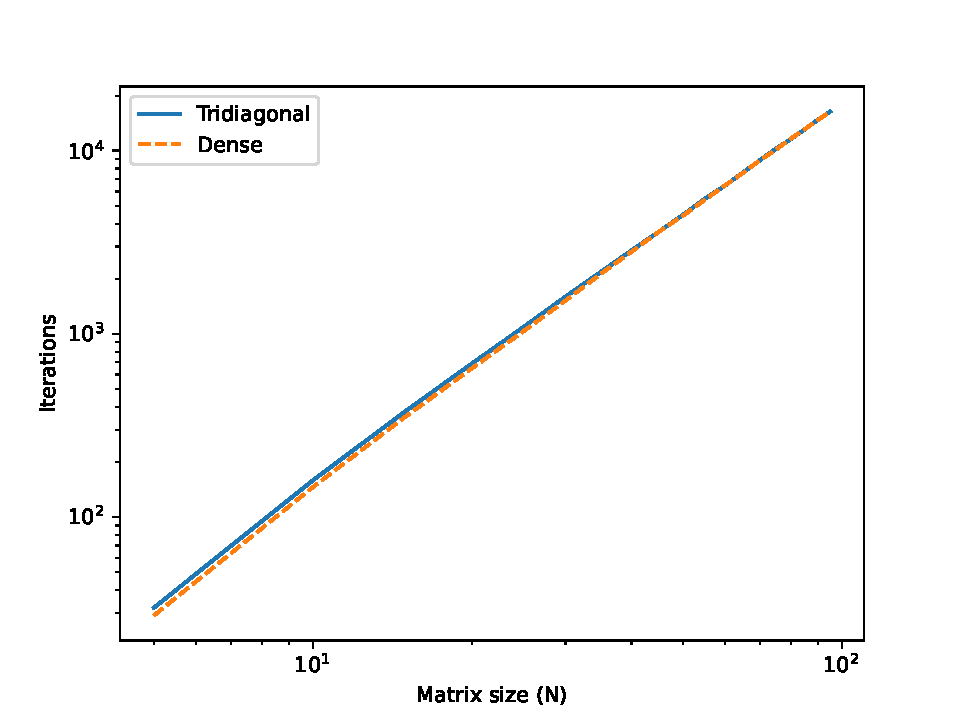
\includegraphics[width=1.\textwidth]{../figures/N_iter_log_both.pdf}
    \caption{The plot shows transformation scaling data for different matrix sizes on a log-log scale. 
    The blue line represents the Jacobi rotation algorithms' behavior for a tridiagonal matrix, 
    whereas the orange line represents the Jacobi rotation algorithms' behavior for a dense matrix.}
    \label{fig:N_iter_log_both}
\end{figure}


\newpage
\section*{Problem 6}
\begin{enumerate}[label= \alph*)]
    \item 
    Solving the equation $\bf{A} \vec{v} = \lambda \vec{v}$ for a discretization 
    of $\hat{x}$ with steps $n = 10$, steps gives us the three eigenvectors in figure
    \ref{fig:eigvec_10}

    \begin{figure}[H]
        \centering
        \begin{subfigure}{.45 \textwidth}
        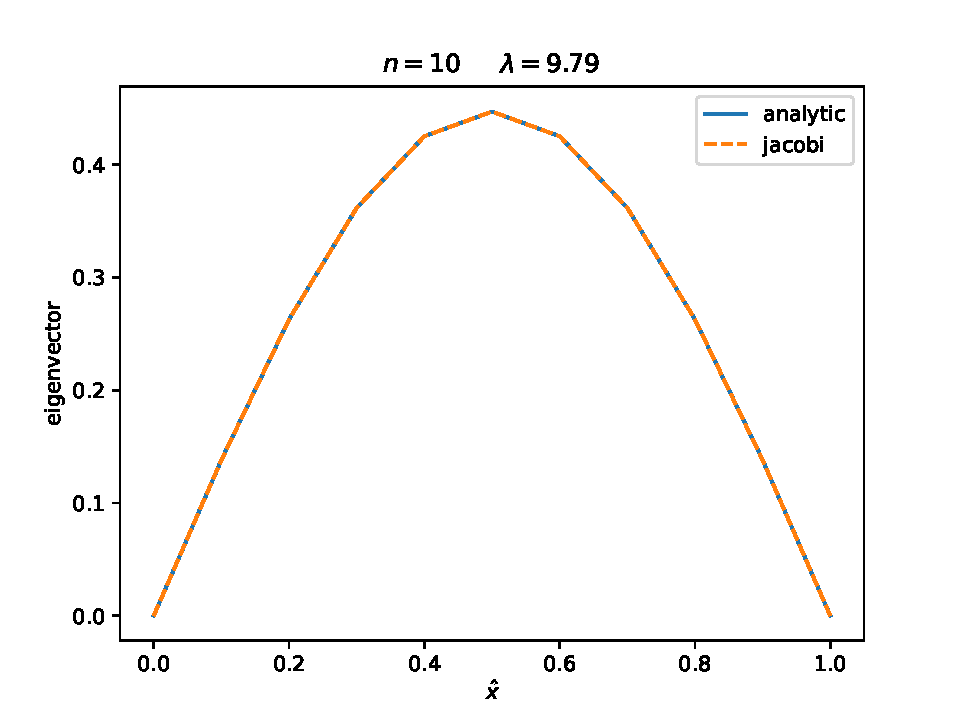
\includegraphics[width=1.1\textwidth]{../figures/eigvec_10_0.pdf}
        \caption{}
        \label{fig:eigvec_10_0}
    \end{subfigure}
    \begin{subfigure}{.45 \textwidth}
        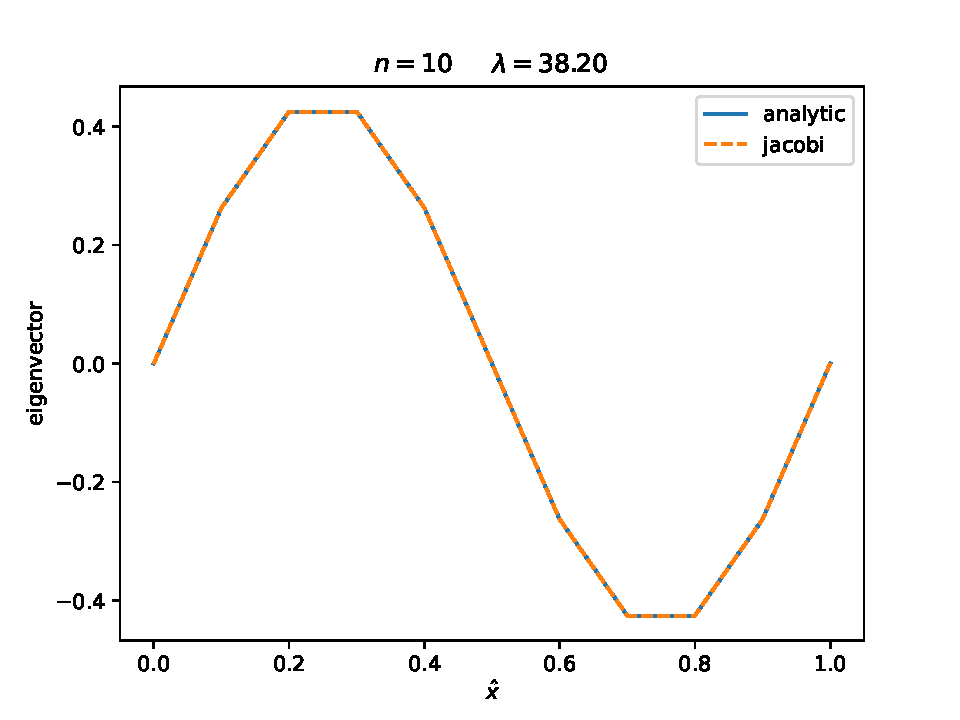
\includegraphics[width=1.1\textwidth]{../figures/eigvec_10_1.pdf}
        \caption{}
        \label{fig:eigvec_10_1}
    \end{subfigure}
    \begin{subfigure}{.45 \textwidth}
        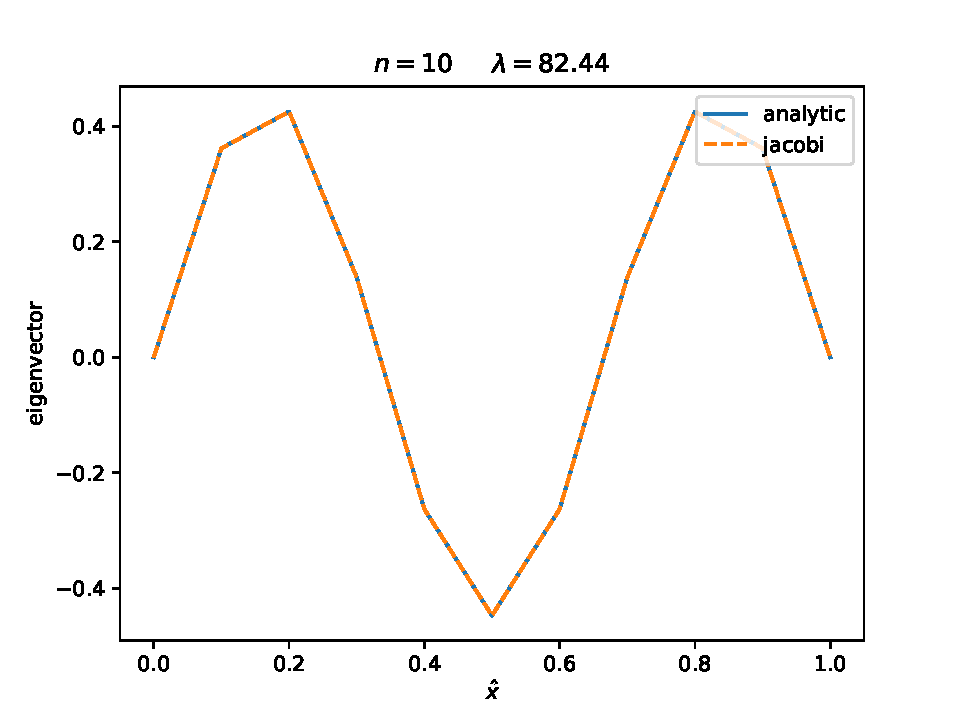
\includegraphics[width=1.1\textwidth]{../figures/eigvec_10_2.pdf}
        \caption{}
        \label{fig:eigvec_10_2}
    \end{subfigure}
    \caption{Eigenvectors corresponding to the three lowest eigenvalues for $n=10$. Plots show the vector $v_i$ elements against the corresponding positions
}
    \label{fig:eigvec_10}
    \end{figure}
\newpage
    \item 
    Figure \ref{fig:eigvec_100} shows the same plots for discretization of with $n = 100$ steps.
    

    \begin{figure}[H]
        \centering
        \begin{subfigure}{.45 \textwidth}
        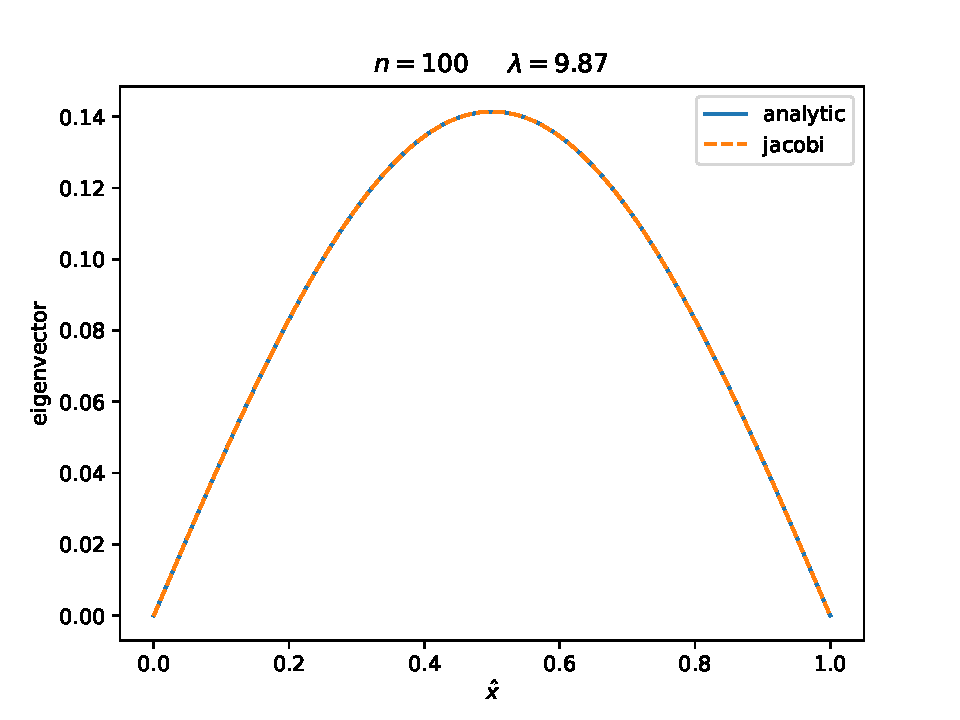
\includegraphics[width=1.1\textwidth]{../figures/eigvec_100_0.pdf}
        \caption{}
        \label{fig:eigvec_100_0}
    \end{subfigure}
    \begin{subfigure}{.45 \textwidth}
        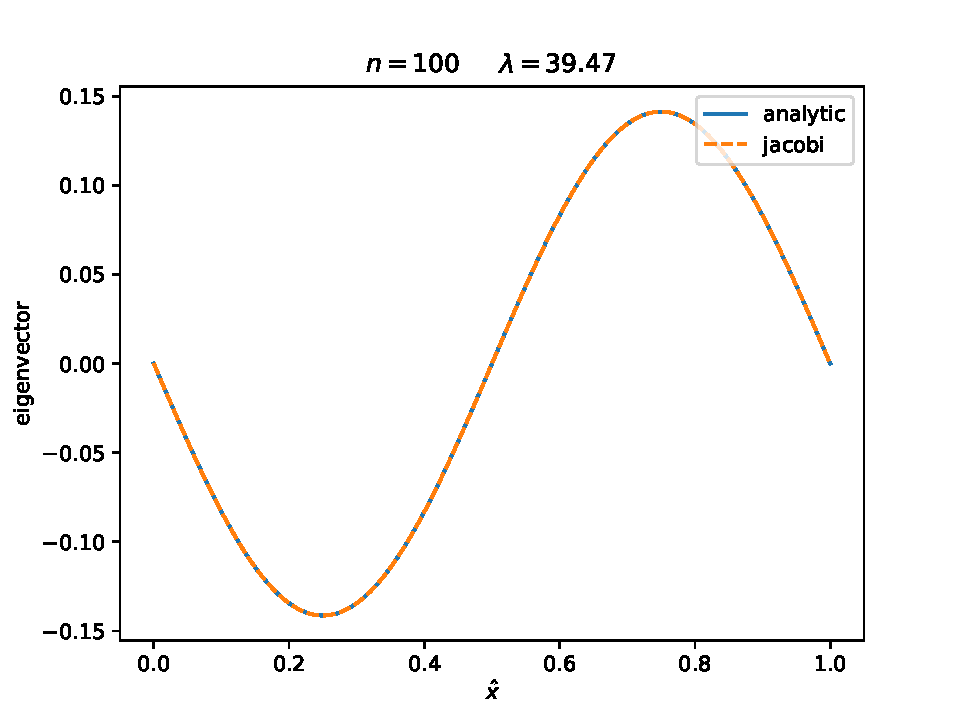
\includegraphics[width=1.1\textwidth]{../figures/eigvec_100_1.pdf}
        \caption{}
        \label{fig:eigvec_100_1}
    \end{subfigure}
    \begin{subfigure}{.45 \textwidth}
        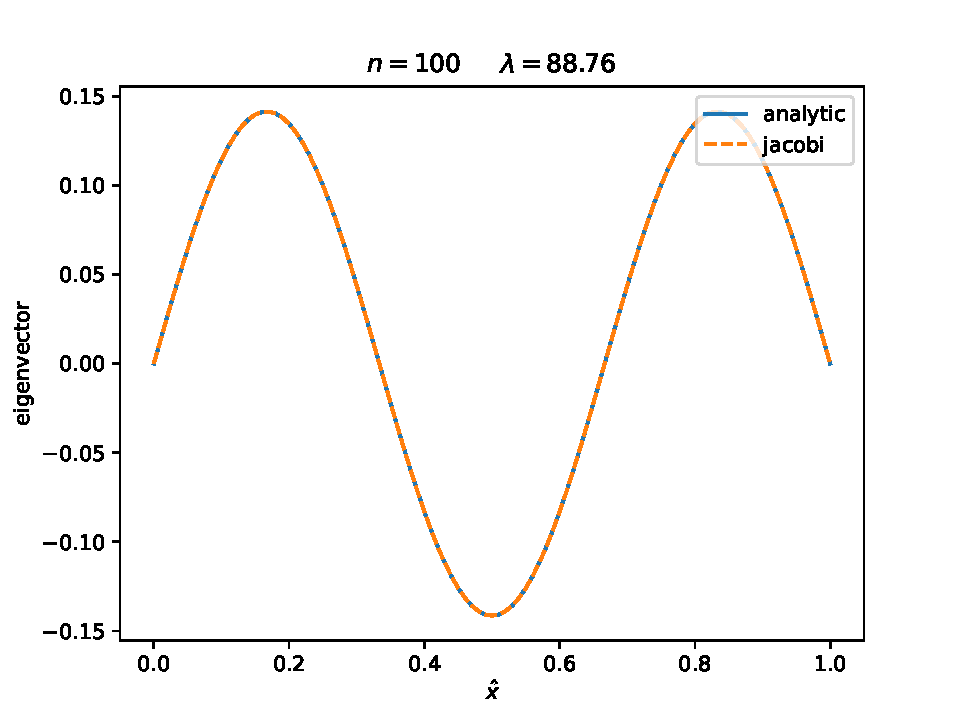
\includegraphics[width=1.1\textwidth]{../figures/eigvec_100_2.pdf}
        \caption{}
        \label{fig:eigvec_100_2}
    \end{subfigure}
    \caption{Eigenvectors corresponding to the three lowest eigenvalues for $n=100$.}
    \label{fig:eigvec_100}
    \end{figure}

\end{enumerate}

\end{document}
